\graphicspath{{../02Physics/pics/}}
	
\chapter[Physics]{Physics}\label{ch:Physics}

\lettrine[lines=2]{\color{darkocre}N}{umbers} are powerful
mathematical objects. They are used to solve
an endless list of problems that involve \emph{quantities}. As
mathematics
and sciences progressed, natural numbers evolved into whole
numbers, then into rational numbers and beyond.\footnote{A superb account of
this process is given in the book \emph{``Number: The Language of
Science''} by Tobias Dantzig.}

\begin{myprereq}{Prerequisite Knowledge}
	To fully understand the material of this chapter, readers should be comfortable with the following concepts:
	
	\begin{itemize}
		\item \phantom{phantom}
		\vspace{-0.5cm}
		\item State
		\item Dynamical equations
	\end{itemize}	
\end{myprereq}

\section{Goals and Methods}
Physics is a \emph{human} activity pursuing the following major goals: \emph{Describe}, \emph{explain}, and \emph{predict} phenomena comprising the observed world.

results can be applied in a wide range of fields. In part, the universality of mathematics
stems from the \emph{general} and \emph{abstract} nature of mathematical
concepts. Let us illustrate this using an example.

\begin{SCfigure}%[htbp]
  %\centering
  
\includegraphics[scale=1.0]{defaultFigureTemplate}
  \caption{49 objects can be arranged in a square 7x7. 48 objects can
    be arranged as a rectangle of 6x8.}
  \label{fig:numbersExampleGenerality}
\end{SCfigure}

An astute farmer notices that 49 sacks of grains can be arranged
in a square with each side having 7 sacks (see the Figure
\ref{fig:numbersExampleGenerality}). When one sack is used up, the
remaining 48 sacks can be arranged as a rectangle 6 by 8 sacks.


\begin{exercise}\label{exe:relationsGeneral}
Think how you would represent the generalized relations of the types
given in the Figure \ref{fig:schematicRelationNtoN} at the level of
sets? What kind of diagrams would you draw?
\end{exercise}

\section{Common Sense}
Mathematics is a remarkably effective and universal discipline, its
methods and
results can be applied in a wide range of fields.
\subsection{Detached Observer}
\begin{figure}[htbp]
	\centering
	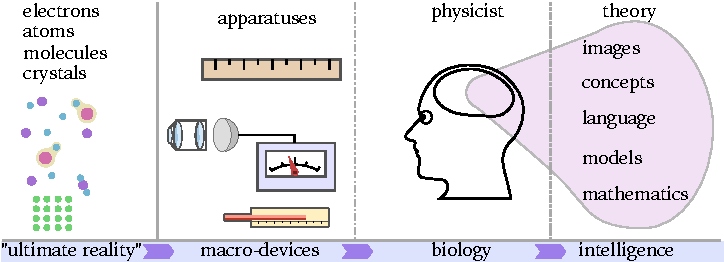
\includegraphics[scale=1.0]{commonSensePerception}
	\caption{Observers in classical view of the world are detached, separated from the "true" reality which they try to comprehend.}
	\label{fig:commonSensePerception}
\end{figure}

\begin{mybio}{Object and Properties}
	Is it possible to separate an object from its properties?
\end{mybio}


\section{Deterministic Evolution}
The completeness of a state is a very strong constraint. Not only it means "everything there is to know at a given moment", but also "know state now -- know state always." The latter is an expression of \emph{determinism}: the complete knowledge of a system is fully determined at all times once an initial state is known. However, state by itself  is not sufficient to satisfy the latter requirement, it must be supplemented by the so called \emph{dynamical equations}. These equations are specific to a physical system and encapsulate the laws that govern internal interactions. EXAMPLE?

Denoting the mathematical representation of the state as $\xi$, the evolution of the state between the moments of time $T=t$ and $T=t+\Delta t$ may be written as a functional dependence:
\[
\xi_{t+\Delta t} = U_{t+\Delta t, t}\,\xi_t\,.
\]
For $\Delta t > 0$ we determine the future state, while for $\Delta t < 0$ we determine the state in the past (relative to the moment $t$).
\begin{myExample}
	For circular motion the state is the angle $\xi=\phi$, and the evolution is given by a simple formula
	\[
	\phi_{t+\Delta t} = U_{t+\Delta t, t}\,\phi_t=\omega \Delta t + \phi_t\,.	
	\]
	Notice that in this case the evolution function depends on the time \emph{difference} $\Delta t$ and not on each moment of time separately:
	\[
	U_{t+\Delta t, t} = U_{\Delta t}\,.
	\]
\end{myExample}
It must be emphasized again, that the final state $\xi_f=\xi_{t+\Delta t}$ is determined by two factors: the initial state $\xi_i=\xi_t$ and the laws of physics encoded in the evolution function $U_{t+\Delta t, t}$. 
\[
\xi_f\, \overset{U_{\Delta t}}{\xleftarrow{\hspace*{2cm}}}\, \xi_i
\]

\begin{figure}[htbp]
	\centering
	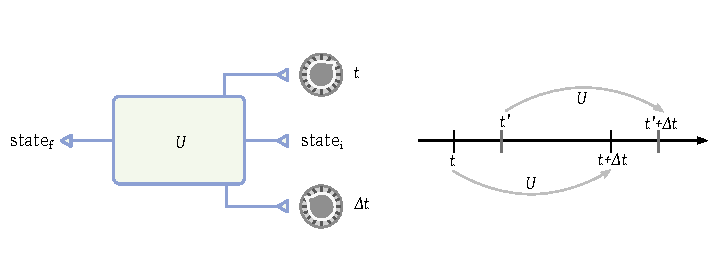
\includegraphics[scale=1.0]{evolutionOperatorBox}
	\caption{Evolution operator transforms an initial state into the final state in time $\Delta t$.}
	\label{fig:evolutionOperatorBox}
\end{figure}

The laws of physics are timeless\footnote{Technical term is \emph{time-translation invariant.}}, as illustrated by the Coulomb's law for the force between charges $q$ and $Q$ at a distance $r$ apart: $F_C=k qQ/r^2$. The timeless nature of the physical laws requires that the same initial state $\xi_i$ evolves into the same final state $\xi_f$ regardless of when the evolution starts as long as the time interval between the beginning and the end of evolution is the same. Mathematically this is expressed as follows:
\[
U_{\tau, t}\,\xi_i  = U_{\tau', t'}\,\xi_i
\]
for \emph{any} initial state $\xi_i$, as long as $\tau'-t'=\tau-t=\Delta t$.

Thus, for \emph{any} values of $t$ and $t'$, we have
\[
U_{t+\Delta t, t}  = U_{t'+\Delta t, t'}\,.
\]
This equation says that the evolution function $U$ becomes insensitive to the values $t$ and $t'$, and only depends on $\Delta t$ -- the time interval between the beginning and the end of evolution. Therefore, we can write the following connection between the states at different moments:
\[
\xi_{t+\Delta t} = U_{\Delta t}\,\xi_t\,.
\]
This connection holds \emph{for any moment of time} $t$ and time interval $\Delta t$.

In physics the states are represented using numbers, vectors, functions, and similar mathematical objects. Common to all of these types of objects is a very basic property of "additivity" and "scalability". That is, one can -- at least formally -- add and subtract states, as well as multiply them by numbers. For example, for any two states $\xi_1$ and $\xi_2$, one can write  equations like
\[
\xi_3 = 2\xi_1 + 3\xi_2\qquad\textrm{ or }\qquad \Delta \xi = \xi_2 - \xi_1\,.
\]

Depending on a particular representation of the state, the evolution function $U$ might be a "usual" function, an operator, or something else entirely. Regardless of what the exact \emph{type} of $U$ is, its job is always the same -- map initial state $\xi_i$ at time $t$ into the final state $\xi_f$ at time $t+\Delta t$.
 
For $\Delta t = 0$ the evolution function $U$ must be a simple \emph{identity} function:
\[
U_0 = I\,.
\]
Furthermore, for a continuous evolution, it is necessary for small changes in time $\delta t$ to produce small changes in the state $\delta \xi$:
\[
\xi_{t+\delta t} = U_{\delta t} \xi_t = \xi_t + \delta \xi\,.
\] 
For a continuous evolution of the state, the evolution function $U$ must be continuous. This implies that for small time intervals it produces small changes:
\[
U_{\delta t} \approx I + \delta U = I + G\delta t\,,
\]
where $G$ is called the \emph{generator} of state evolution. The meaning of the generator is clear from its definition -- it specifies how fast the state evolution happens: $G=\partial_t U$.

In terms of the generator, the evolution equation can be written using the relations 
\[
\delta \xi = \xi_{t+\delta t} - \xi_t = \left(I + G\delta t\right)\xi_t - \xi_t = G\delta t\xi_t\,.
\]
Finally, dividing both sides by $\delta t$ and using the $\partial$-notation, we arrive at the Schrodinger-type of equation for the \emph{continuous} state evolution:
\begin{equation}
	\partial_t \xi = G\,\xi_t\,.
	\label{eq:SchrodingerTypeEq}
\end{equation}
The equation (\ref{eq:SchrodingerTypeEq}) is a general form of state evolution equations used in physics. It appears in many cases where the dynamics of a system is described as a \emph{continuous deterministic evolution}. 
\begin{mybio}{Deterministic Evolution Equations}
	Equations similar to (\ref{eq:SchrodingerTypeEq}) can be found in many physical theories. In quantum theory it is Schrodinger equation, which can be written as follows:
	\[
	\partial_t\ket{\Psi} = -i\hat{H}\,\ket{\Psi}\,.
	\]
\end{mybio}


\section{Classical and Quantum}
Mathematics is a remarkably effective and universal discipline, its
methods and
results can be applied in a wide range of fields.

\section{State}
State is a very important concept in physics. It means \emph{complete} but \emph{minimal} knowledge about  possible behavior of a given system.
\begin{figure}[htbp]
	\centering
	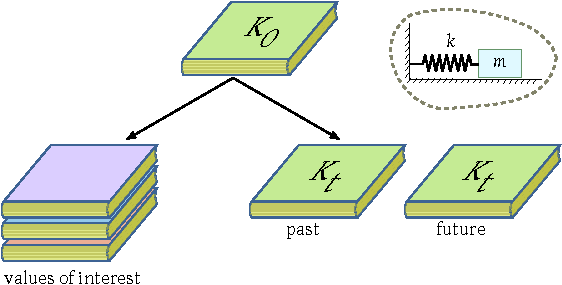
\includegraphics[scale=1.0]{stateAsKnowledge}
	\caption{State is a minimal and complete knowledge about a physical system.}
	\label{fig:stateAsKnowledge}
\end{figure}
By \emph{minimal} knowledge we mean that if position of particle $x$ is known, there is no need to know $x^3$ or any other one-to-one function of position. We only need to know and keep track of the \emph{essential} information.

\begin{mybio}{Completeness}
	How can we be sure that the information about a system is complete? Can there be some "hidden" information, unaccessible (may be yet, or even potentially forever) to us and yet affecting the behavior of a system?
	
	The question of completeness is an important one. In the context of quantum physics it was raised for the first time by Albert Einstein, Boris Podolsky, and Nathan Rosen in 1935.
\end{mybio}

\section{Measurement}
Measurement is the source of our knowledge about the world. This is true for both classical and quantum physics. 
\begin{figure}[htbp]
	\centering
	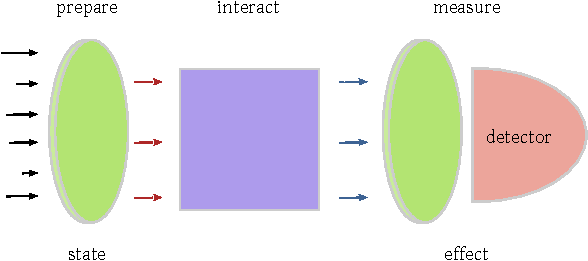
\includegraphics[scale=1.0]{measurementStages}
	\caption{Three stages of measurement process: Preparation of a system in a certain state, followed by the interaction of the system with external system, ending with the measurement which extract the information.}
	\label{fig:measurementStages}
\end{figure}

\subsection{Joint Measurement}
Imagine you put your left hand and right hand on different pads and discover that both hands move up and down randomly but in total sync.

\section{Atoms}
Classical physics predicts a continuous decay of unstable configuration of charges. What is observed is a spontaneous decay of stable configuration of charges. Quantum physics elegantly explains the latter.  

\section{Particles}
Classical physics predicts a continuous decay of unstable configuration of charges. What is observed is a spontaneous decay of stable configuration of charges. Quantum physics elegantly explains the latter.  
\subsection{Photon And Electron}
Two types of fundamental elementary particles that will be discussed in this book are photons and electrons.

\section{Avalanche Detectors}
The dominant way humans perceive the world is through the eyesight. 

\subsection{Quantum Eyes}
The first time physicists heard an effect due to a single particle (alpha-particle) was in 19xx in an experiment performed by Ernst Rutherford and Heiger.


\section{Polarization and Spin}
Mathematics is a remarkably effective and universal discipline, its
methods and
results can be applied in a wide range of fields.

% ---------------------- Chapter Highlights -------------------------------
\section*{Chapter Highlights}
{\setstretch{1.5}\chhc
  \it  
\begin{itemize}
\item The power of mathematical concepts and methods increases with
  the level of abstraction.
\item Learning new concepts often involves learning new
  terminology. The latter can create an artificial mental barrier.
\item ``Usual'' numbers form a mathematical structure. The structure
  is revealed through various relations that exist between numbers.
\item Relations between numbers are expressed using the concept of
  functions and operations (e.g., addition). Each operation is
  characterized by its arity -- the number of arguments it accepts as
  an input.
\end{itemize}


}
